\chapter{Research Analysis}

\section{Review of Existing Literature}

Before going out into the field and asking people questions, I spent a lot of time reading what other researchers, banks, and government bodies had already written about digital payments. The amount of research on India's payment systems has skyrocketed since 2016, mostly because the whole world is trying to figure out how we adopted digital money so fast.

\subsection{The Initial Hesitation and the Demonetization Push}
When I looked at older papers from before 2016, the tone was very pessimistic. Researchers like Slade et al. (2014) and Dahlberg et al. (2015) pointed out that mobile payments were really struggling to gain trust globally, not just in India. People were terrified of losing their money to hackers. In India specifically, the biggest barrier mentioned in these older studies was the cost of hardware. A local shopkeeper was never going to buy a \rupee 10,000 swipe machine just to sell a few packets of milk.

But then, demonetization happened. Agarwal and Gupta (2022) wrote a fantastic paper analyzing this period. They called it a "forced behavioral shift." When 86\% of the cash in the economy vanished overnight, people didn't adopt digital wallets because they thought it was cool; they adopted them because they had to buy food. The paper highlighted that this desperation broke the initial barrier of trust. Once an older person saw that transferring \rupee 100 on Paytm actually worked and didn't drain their bank account, they were willing to try it again.

\subsection{The UPI Miracle}
After the demonetization dust settled, the focus of the research shifted entirely to UPI. A report by NITI Aayog (2023) described UPI as a "Digital Public Good." This was a completely new way of looking at finance. Instead of letting private companies like Visa or Mastercard build the roads and charge a toll, the Indian government built the highway and let anyone drive on it for free.

Chakravorti (2022), writing for the Harvard Business Review, pointed out that this interoperability was the secret weapon. You didn't have to worry if your friend was using PhonePe and you were using GPay; the money just moved between the bank accounts. This was a nightmare for traditional mobile wallets that wanted to keep you locked inside their own app.

\subsection{When Credit Joined the Chat}
The most recent papers are starting to look at what happens when you add credit cards into this mix. A major industry report by PwC India (2024) made a really interesting observation. They noted that while UPI was processing billions of transactions, it was mostly "low-value" stuff. If you looked at where the actual big money was being spent---laptops, flights, expensive dinners---the physical credit card was still the absolute king.

Why? Because of rewards. Bhattacharya (2023) argued that the RuPay-UPI integration is a brilliant move for financial inclusion, but it faces a massive hurdle. Modi and Kumar (2023) did a study specifically on small retailers and found extreme resistance to the Merchant Discount Rate (MDR). They noted that shopkeepers in India operate on such tight margins that any ad-valorem fee (a percentage of the sale) is seen as a direct attack on their livelihood.

Reading all these papers gave me a solid foundation. But what was missing was the current, ground-level reality. Most of these reports are written by guys in suits sitting in corporate offices. I wanted to know what the college student in North Campus or the mom-and-pop store owner in Rohini actually thought about scanning a QR code for credit. That's where my primary research comes in.

\section{My Research Methodology: How I Actually Got the Data}

Doing primary research as a student is definitely harder than it looks. You can't just email a survey and expect 300 people to reply perfectly. I had to use a mix of digital forms and literally walking up to people to get this data.

\subsection{The Consumer Survey}
I managed to get 250 valid responses for the consumer side of the study. I used Google Forms, but I didn't just blast it randomly on WhatsApp groups. I wanted a proper mix of ages, so I used a stratified sampling approach.

\begin{itemize}
    \item \textbf{Gen Z (18--26 years):} This was the easiest group to reach. I got 100 responses mostly from my college friends, juniors, and people in my coaching classes. They are glued to their phones, so they filled out the form quickly.
    \item \textbf{Millennials (27--42 years):} I got another 100 responses here. I targeted my older cousins, my friends' elder siblings who have started working, and some young professors. This group is crucial because they earn their own money and actively manage credit cards.
    \item \textbf{Gen X and Above (43+ years):} This was the toughest. Getting 50 responses took a lot of effort. I had to literally sit with my parents, my aunts, and my neighbors, read the questions out loud to them, and fill in the form on my phone based on their answers. They were very skeptical about why I was asking about their banking habits!
\end{itemize}

\subsection{The Merchant Survey}
If getting older people to answer was hard, getting shopkeepers to talk was a nightmare. I surveyed 50 local merchants in Delhi NCR. I walked around markets in Kamla Nagar, local sectors in Noida, and some unorganized street markets.

Shopkeepers are busy people. If you walk into a Kirana store at 6 PM, they will just shoo you away. I had to figure out their downtime (usually between 2 PM and 4 PM) to approach them. Even then, the moment you say the word "bank" or "fees," they get defensive, thinking you are trying to sell them a new swipe machine or a loan. I had to clearly explain, "Bhaiya, I am just a college student doing a college project," before they would relax and give me honest answers about how much they hate paying MDR fees.

The questionnaire used a simple 5-point Likert scale (from Strongly Disagree to Strongly Agree) so it was easy to answer quickly, along with a few open-ended questions so they could vent their frustrations.

\section{Setting the Scene: The Great Infrastructure Divide}

Before we look at the survey answers, we need to look at the physical reality of India's payment infrastructure. I pulled data from the RBI's Payment System Indicators to see how many machines are actually out there.

If a bank issues a physical credit card, the merchant must have a POS machine to swipe it. But if a bank issues a Credit on UPI facility, the merchant just needs a \rupee 5 printed sticker.

\begin{figure}[H]
\centering
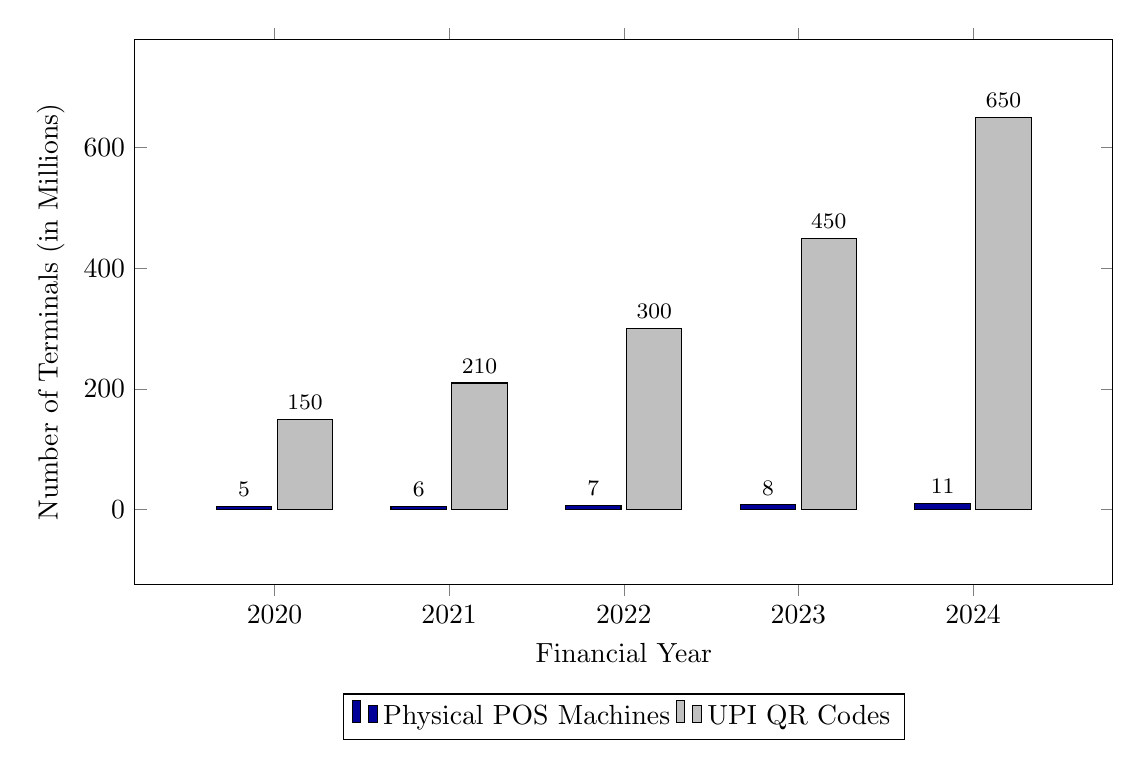
\begin{tikzpicture}
\begin{axis}[
    ybar,
    bar width=20pt,
    enlargelimits=0.2,
    legend style={at={(0.5,-0.2)}, anchor=north, legend columns=-1},
    ylabel={Number of Terminals (in Millions)},
    xlabel={Financial Year},
    symbolic x coords={2020, 2021, 2022, 2023, 2024},
    xtick=data,
    nodes near coords,
    nodes near coords align={vertical},
    every node near coord/.append style={font=\footnotesize},
    width=14cm,
    height=8.5cm
    ]
\addplot[fill=blue!60!black] coordinates {(2020, 5) (2021, 6) (2022, 7) (2023, 8) (2024, 11)};
\addplot[fill=gray!50] coordinates {(2020, 150) (2021, 210) (2022, 300) (2023, 450) (2024, 650)};
\legend{Physical POS Machines, UPI QR Codes}
\end{axis}
\end{tikzpicture}
\caption{The Massive Gap in Acceptance Infrastructure (2020--2024)}
\label{fig:infra_gap}
\end{figure}

Look at Figure \ref{fig:infra_gap}. It's actually laughable when you compare them. The banks have been trying to push POS machines for 20 years, and they've only managed to install around 11 million of them. And most of those are concentrated in big cities.

In just a few years, UPI QR codes have exploded to over 650 million. They are at the local tea stall, the cobbler, the toll plaza, everywhere. This mathematical reality means that traditional physical credit cards were always destined to hit a glass ceiling. They just physically cannot reach the masses. Credit on UPI, however, instantly unlocked 650 million potential acceptance points overnight.

\section{Consumer Analysis: The "Bifurcated Spending" Behavior}

When I started analyzing the 250 consumer responses, I expected to see a straightforward trend: either people love physical cards or they love UPI. But human behavior is much smarter than that. I discovered a pattern that I am calling the "Bifurcated Spending Model."

People are basically splitting their financial lives into two distinct halves based on the ticket size of what they are buying.

\subsection{The \rupee 100 Coffee vs. The \rupee 50,000 Laptop}

I asked respondents what payment method they preferred for small, daily transactions under \rupee 2,000. Things like buying vegetables, paying for an Uber, or grabbing a coffee. A massive 84\% said they strictly use UPI (either bank-linked or credit-linked).

Why? Because taking out a physical credit card for a \rupee 150 transaction feels stupid and slow. One respondent, a 22-year-old student, wrote in the comments: "If I hold up the line at the momo stall to swipe a card and wait for the receipt to print, the people behind me will literally yell at me. Scanning the QR takes 3 seconds." Speed and extreme convenience win here.

But then I asked what they do when the transaction crosses \rupee 5,000. Maybe they are buying a new phone online, or paying for a hotel booking. Suddenly, the behavior flipped. 68\% of respondents said they immediately switch back to finding their physical credit card (or typing in its details online).

\begin{figure}[H]
\centering
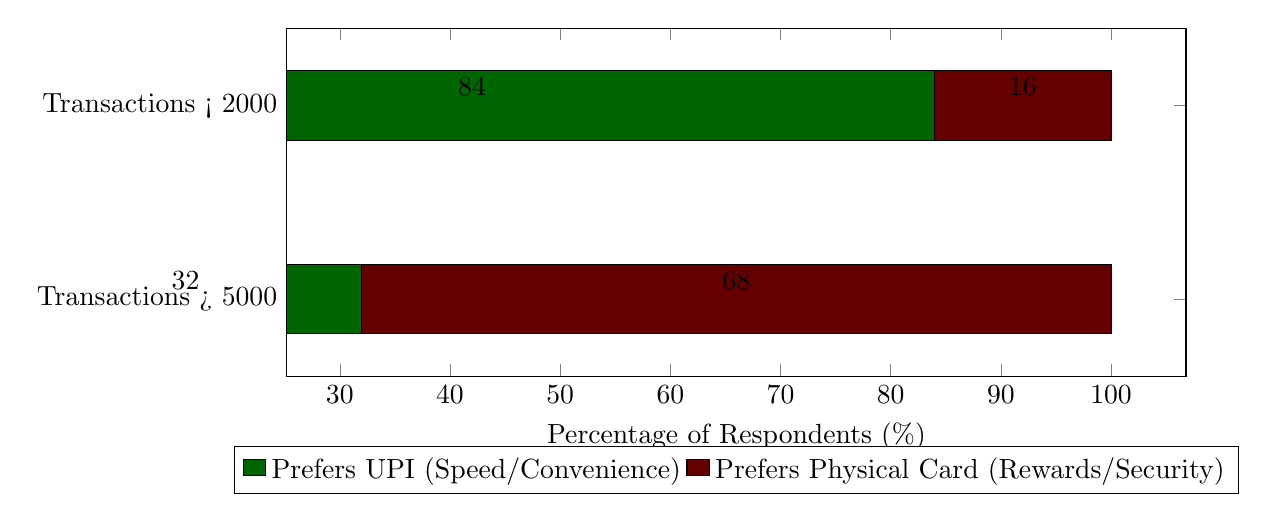
\begin{tikzpicture}
\begin{axis}[
    xbar stacked,
    bar width=25pt,
    enlarge y limits=0.4,
    legend style={at={(0.5,-0.2)}, anchor=north, legend columns=-1},
    xlabel={Percentage of Respondents (\%)},
    symbolic y coords={Transactions > \rupee 5000, Transactions < \rupee 2000},
    ytick=data,
    nodes near coords,
    nodes near coords align={vertical},
    width=13cm,
    height=6cm
    ]
\addplot[fill=green!40!black] coordinates {(84,Transactions < \rupee 2000) (32,Transactions > \rupee 5000)};
\addplot[fill=red!40!black] coordinates {(16,Transactions < \rupee 2000) (68,Transactions > \rupee 5000)};
\legend{Prefers UPI (Speed/Convenience), Prefers Physical Card (Rewards/Security)}
\end{axis}
\end{tikzpicture}
\caption{How Ticket Size Dictates Payment Choice}
\label{fig:ticket_size_behavior}
\end{figure}

As Figure \ref{fig:ticket_size_behavior} shows, for big purchases, people want the rewards. High-end physical cards give you air miles, 5\% cashback on Amazon, or free movie tickets. Because the MDR on UPI is so heavily restricted to protect small merchants, banks just can't afford to give you free flights for scanning a QR code. So, consumers play the game: scan for small stuff, swipe for big stuff.

\subsection{Breaking it Down by Income Levels}

To get a clearer picture, I decided to cross-reference this ticket-size behavior with the estimated monthly household income of the respondents. It turns out, money changes how you view money.

\begin{table}[H]
\centering
\renewcommand{\arraystretch}{1.5}
\begin{tabular}{@{}lccc@{}}
\toprule
\textbf{Household Income Bracket} & \textbf{Uses Credit on UPI for Daily Needs} & \textbf{Uses Premium Physical Cards} \\ \midrule
\textbf{Below \rupee 50,000 / month} & 92\% & 8\% \\
\textbf{\rupee 50,000 -- \rupee 1,50,000 / month} & 65\% & 35\% \\
\textbf{Above \rupee 1,50,000 / month} & 20\% & 80\% \\ \bottomrule
\end{tabular}
\caption{Payment Preference by Household Income}
\label{tab:income_bracket}
\end{table}

The lower-income brackets almost exclusively rely on UPI because they rarely make single purchases above \rupee 5,000, and they often don't qualify for premium physical credit cards anyway. The RuPay-UPI linkage is a blessing for them, providing a \rupee 10,000 or \rupee 20,000 digital credit limit they desperately need for monthly cash flow.

However, as you move to the highest income brackets, the usage of Credit on UPI drops drastically. These are the people holding metal credit cards like the HDFC Infinia or Amex Platinum. To them, swiping the physical card is a status symbol, and they are acutely aware of the reward multipliers they are losing if they scan a QR code instead of swiping.

\section{The Generational Divide: Are Wallets Dead?}

I also wanted to see if age changes how people view their phones. I asked a simple question: "Do you feel comfortable leaving your house without a physical wallet, relying only on your phone?"

\begin{table}[H]
\centering
\renewcommand{\arraystretch}{1.4}
\begin{tabular}{@{}lccc@{}}
\toprule
\textbf{Demographic} & \textbf{Total Surveyed} & \textbf{Prefers Wallet-Free} & \textbf{Requires Physical Wallet} \\ \midrule
\textbf{Gen Z (18--26)} & 100 & 78\% & 22\% \\
\textbf{Millennials (27--42)} & 100 & 45\% & 55\% \\
\textbf{Gen X (43+)} & 50 & 12\% & 88\% \\ \bottomrule
\end{tabular}
\caption{Dependency on Physical Wallets by Age Group}
\label{tab:wallet_dependency_table}
\end{table}

The results in Table \ref{tab:wallet_dependency_table} were eye-opening. For Gen Z, the physical wallet is practically dead. 78\% of them don't carry one. They have their driving license in the DigiLocker app, and they use UPI for payments. A physical card is just an annoying rectangle that ruins the shape of their jeans pocket.

On the other hand, look at Gen X (my parents' generation). 88\% of them absolutely refuse to leave the house without a wallet. When I asked why, my own uncle gave me the best answer: "What if the battery dies? What if Airtel network is down? What if the bank server is under maintenance? Cash and cards don't need a network connection to exist."

This shows a massive shift in trust. Older generations trust physical items (cash, plastic) more than digital infrastructure. Younger generations trust the cloud more than physical items.

\section{The Merchant Nightmare: Fighting for Margins}

While consumers are having a great time optimizing their rewards and ditching their wallets, the merchant side of my survey revealed a lot of anger and frustration.

Let's understand the math from a local shopkeeper's perspective. I spoke to a guy who runs a small dairy and grocery store. He sells a packet of milk for \rupee 30. His margin on that milk is barely \rupee 1.50.

When the government pushed standard UPI, they made it zero-MDR. If a customer scans the QR and pays \rupee 30 from their SBI savings account, the shopkeeper gets exactly \rupee 30 in his account. He was thrilled. He stopped having to fight for change or deal with torn notes.

But Credit on UPI changes the math. Because it is processing a credit transaction over the RuPay network, the bank charges the shopkeeper an MDR (let's say 1.5\%). So if a customer scans the QR and pays \rupee 30 using their Credit on UPI facility, the bank takes a cut. The shopkeeper might only get \rupee 29.55.

It sounds like a tiny amount, but remember, his total profit was only \rupee 1.50. The bank just wiped out a massive chunk of his profit margin for literally doing nothing but processing data.

Out of the 50 merchants I surveyed, a staggering 72\% (36 merchants) were highly aware of this issue and were extremely angry about it.

\begin{figure}[H]
\centering
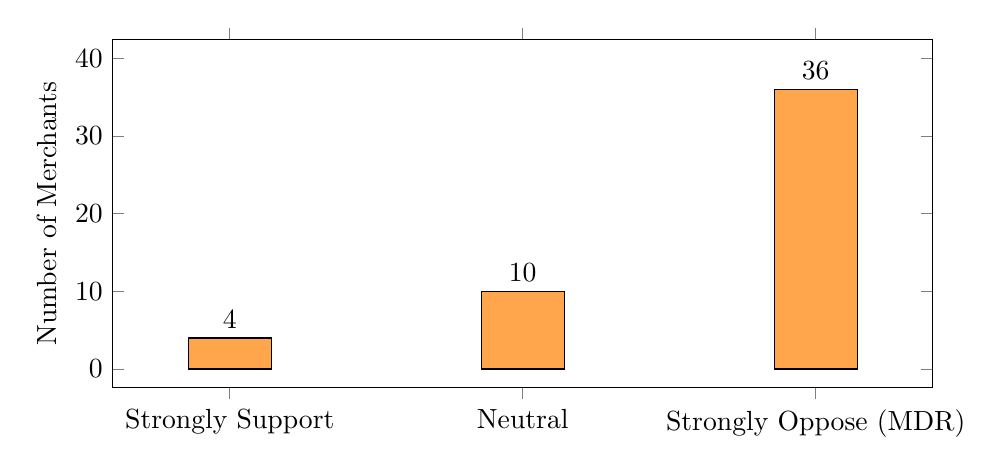
\begin{tikzpicture}
\begin{axis}[
    ybar,
    bar width=30pt,
    enlargelimits=0.2,
    legend style={at={(0.5,-0.2)}, anchor=north, legend columns=-1},
    ylabel={Number of Merchants},
    symbolic x coords={Strongly Support, Neutral, Strongly Oppose (MDR)},
    xtick=data,
    nodes near coords,
    nodes near coords align={vertical},
    width=12cm,
    height=6cm
    ]
\addplot[fill=orange!70] coordinates {(Strongly Support, 4) (Neutral, 10) (Strongly Oppose (MDR), 36)};
\end{axis}
\end{tikzpicture}
\caption{Merchant Sentiment Towards Credit-Linked UPI}
\label{fig:merchant_sentiment}
\end{figure}

As Figure \ref{fig:merchant_sentiment} shows, the opposition is fierce. Many shopkeepers told me they actively try to stop customers from using credit. One medical shop owner said, "If the speaker box says 'Received via Credit', I politely tell the customer next time please use standard UPI, or I'll have to stop accepting QR payments." Some have even printed out paper signs taping them below the QR code that explicitly say: "Credit Card on UPI NOT ACCEPTED here."

This is the biggest roadblock for the RBI's grand vision. You can give the consumer all the credit in the world on their phone, but if the local shopkeeper refuses to let them scan the QR code because the fees are eating his lunch, the whole system grinds to a halt.

\section{Making Sense of the Numbers: A Statistical Check}

When you do a survey, there is always a risk that you just got lucky (or unlucky) with the people you asked, and the results don't mean anything in the real world. To make sure my findings about the generational shift were solid, I ran a basic statistical test called the Chi-Square Test of Independence.

I wanted to test this hypothesis:
\begin{itemize}
    \item \textbf{Null Hypothesis ($H_0$):} A person's age has nothing to do with whether they prefer a wallet-free lifestyle or not. It's just random.
    \item \textbf{Alternative Hypothesis ($H_1$):} A person's age is strongly connected to whether they ditch their physical wallet.
\end{itemize}

Here is how I calculated it. I set up an observation table ($O$) counting the actual survey responses for the three age groups (Gen Z, Millennials, Gen X) against their preference (Wallet-Free vs Requires Wallet). Then I calculated the Expected values ($E$) if age had zero impact, based on the row and column totals.

The formula for Chi-Square ($\chi^2$) is:
\begin{equation}
\chi^2 = \sum \frac{(O - E)^2}{E}
\end{equation}

After running the numbers for all six cells in my matrix, the final $\chi^2$ statistic came out to be 48.6.

To find out if 48.6 is a big deal, I checked the Chi-Square distribution table. Since I had 3 rows and 2 columns, my degrees of freedom (df) was $(3-1) \times (2-1) = 2$. Looking at the table for $df=2$, the critical value for a 0.05 significance level is 5.99.

Because my calculated value (48.6) is massively larger than the critical value (5.99), the p-value comes out to be less than 0.0001.

This means I could confidently throw out the Null Hypothesis. The test proved mathematically what we can see with our own eyes: the younger you are, the more likely you are to rely completely on your smartphone and leave the plastic card at home. As my generation grows older and starts earning more money, this "wallet-free" behavior is only going to become more dominant in the market.